% Created by tikzDevice version 0.10.1 on 2018-06-21 09:35:15
% !TEX encoding = UTF-8 Unicode
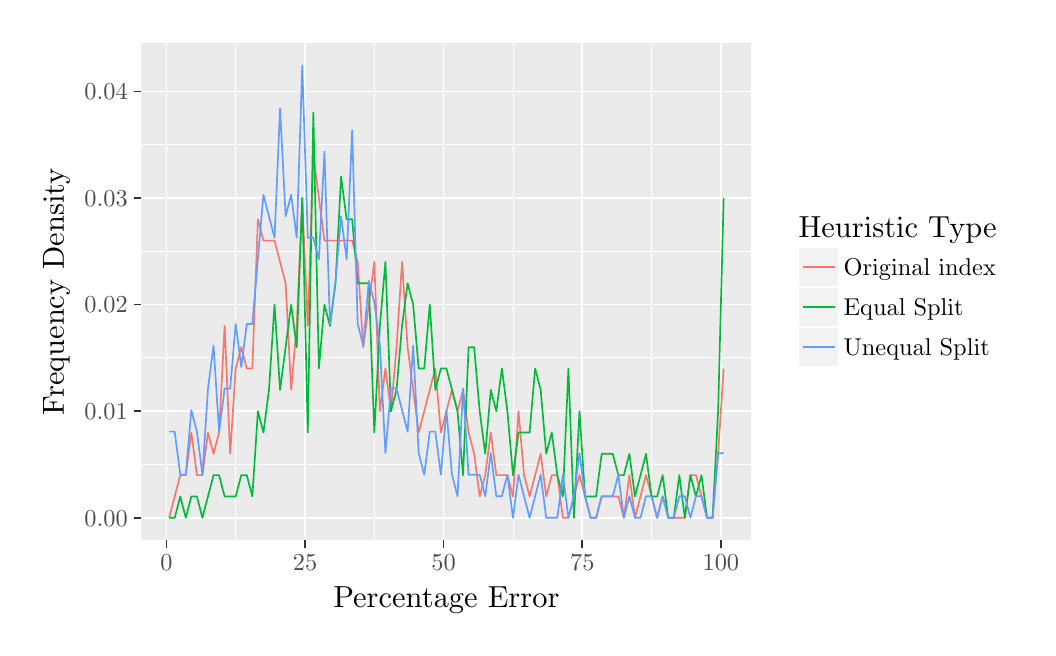
\begin{tikzpicture}[x=1pt,y=1pt]
\definecolor{fillColor}{RGB}{255,255,255}
\path[use as bounding box,fill=fillColor,fill opacity=0.00] (0,0) rectangle (361.35,216.81);
\begin{scope}
\path[clip] (  0.00,  0.00) rectangle (361.35,216.81);
\definecolor{drawColor}{RGB}{255,255,255}
\definecolor{fillColor}{RGB}{255,255,255}

\path[draw=drawColor,line width= 0.6pt,line join=round,line cap=round,fill=fillColor] (  0.00,  0.00) rectangle (361.35,216.81);
\end{scope}
\begin{scope}
\path[clip] ( 41.11, 31.53) rectangle (261.51,211.31);
\definecolor{fillColor}{gray}{0.92}

\path[fill=fillColor] ( 41.11, 31.53) rectangle (261.51,211.31);
\definecolor{drawColor}{RGB}{255,255,255}

\path[draw=drawColor,line width= 0.3pt,line join=round] ( 41.11, 58.96) --
	(261.51, 58.96);

\path[draw=drawColor,line width= 0.3pt,line join=round] ( 41.11, 97.49) --
	(261.51, 97.49);

\path[draw=drawColor,line width= 0.3pt,line join=round] ( 41.11,136.01) --
	(261.51,136.01);

\path[draw=drawColor,line width= 0.3pt,line join=round] ( 41.11,174.54) --
	(261.51,174.54);

\path[draw=drawColor,line width= 0.3pt,line join=round] ( 75.17, 31.53) --
	( 75.17,211.31);

\path[draw=drawColor,line width= 0.3pt,line join=round] (125.26, 31.53) --
	(125.26,211.31);

\path[draw=drawColor,line width= 0.3pt,line join=round] (175.36, 31.53) --
	(175.36,211.31);

\path[draw=drawColor,line width= 0.3pt,line join=round] (225.45, 31.53) --
	(225.45,211.31);

\path[draw=drawColor,line width= 0.6pt,line join=round] ( 41.11, 39.70) --
	(261.51, 39.70);

\path[draw=drawColor,line width= 0.6pt,line join=round] ( 41.11, 78.23) --
	(261.51, 78.23);

\path[draw=drawColor,line width= 0.6pt,line join=round] ( 41.11,116.75) --
	(261.51,116.75);

\path[draw=drawColor,line width= 0.6pt,line join=round] ( 41.11,155.27) --
	(261.51,155.27);

\path[draw=drawColor,line width= 0.6pt,line join=round] ( 41.11,193.80) --
	(261.51,193.80);

\path[draw=drawColor,line width= 0.6pt,line join=round] ( 50.13, 31.53) --
	( 50.13,211.31);

\path[draw=drawColor,line width= 0.6pt,line join=round] (100.22, 31.53) --
	(100.22,211.31);

\path[draw=drawColor,line width= 0.6pt,line join=round] (150.31, 31.53) --
	(150.31,211.31);

\path[draw=drawColor,line width= 0.6pt,line join=round] (200.40, 31.53) --
	(200.40,211.31);

\path[draw=drawColor,line width= 0.6pt,line join=round] (250.49, 31.53) --
	(250.49,211.31);
\definecolor{drawColor}{RGB}{248,118,109}

\path[draw=drawColor,line width= 0.6pt,line join=round] ( 51.13, 39.70) --
	( 53.13, 47.41) --
	( 55.14, 55.11) --
	( 57.14, 55.11) --
	( 59.14, 70.52) --
	( 61.15, 55.11) --
	( 63.15, 55.11) --
	( 65.15, 70.52) --
	( 67.16, 62.82) --
	( 69.16, 70.52) --
	( 71.17,109.05) --
	( 73.17, 62.82) --
	( 75.17, 93.64) --
	( 77.18,101.34) --
	( 79.18, 93.64) --
	( 81.18, 93.64) --
	( 83.19,147.57) --
	( 85.19,139.87) --
	( 87.19,139.87) --
	( 89.20,139.87) --
	( 91.20,132.16) --
	( 93.21,124.46) --
	( 95.21, 85.93) --
	( 97.21,109.05) --
	( 99.22,155.27) --
	(101.22,109.05) --
	(103.22,170.68) --
	(105.23,155.27) --
	(107.23,139.87) --
	(109.24,139.87) --
	(111.24,139.87) --
	(113.24,139.87) --
	(115.25,139.87) --
	(117.25,139.87) --
	(119.25,132.16) --
	(121.26,101.34) --
	(123.26,116.75) --
	(125.26,132.16) --
	(127.27, 78.23) --
	(129.27, 93.64) --
	(131.28, 78.23) --
	(133.28,101.34) --
	(135.28,132.16) --
	(137.29,101.34) --
	(139.29, 85.93) --
	(141.29, 70.52) --
	(143.30, 78.23) --
	(145.30, 85.93) --
	(147.30, 93.64) --
	(149.31, 70.52) --
	(151.31, 78.23) --
	(153.32, 85.93) --
	(155.32, 78.23) --
	(157.32, 85.93) --
	(159.33, 70.52) --
	(161.33, 62.82) --
	(163.33, 47.41) --
	(165.34, 55.11) --
	(167.34, 70.52) --
	(169.34, 55.11) --
	(171.35, 55.11) --
	(173.35, 55.11) --
	(175.36, 47.41) --
	(177.36, 78.23) --
	(179.36, 55.11) --
	(181.37, 47.41) --
	(183.37, 55.11) --
	(185.37, 62.82) --
	(187.38, 47.41) --
	(189.38, 55.11) --
	(191.39, 55.11) --
	(193.39, 39.70) --
	(195.39, 39.70) --
	(197.40, 47.41) --
	(199.40, 55.11) --
	(201.40, 47.41) --
	(203.41, 39.70) --
	(205.41, 39.70) --
	(207.41, 47.41) --
	(209.42, 47.41) --
	(211.42, 47.41) --
	(213.43, 47.41) --
	(215.43, 39.70) --
	(217.43, 55.11) --
	(219.44, 39.70) --
	(221.44, 47.41) --
	(223.44, 55.11) --
	(225.45, 47.41) --
	(227.45, 39.70) --
	(229.45, 47.41) --
	(231.46, 39.70) --
	(233.46, 39.70) --
	(235.47, 39.70) --
	(237.47, 39.70) --
	(239.47, 55.11) --
	(241.48, 55.11) --
	(243.48, 47.41) --
	(245.48, 39.70) --
	(247.49, 39.70) --
	(249.49, 62.82) --
	(251.49, 93.64);
\definecolor{drawColor}{RGB}{0,186,56}

\path[draw=drawColor,line width= 0.6pt,line join=round] ( 51.13, 39.70) --
	( 53.13, 39.70) --
	( 55.14, 47.41) --
	( 57.14, 39.70) --
	( 59.14, 47.41) --
	( 61.15, 47.41) --
	( 63.15, 39.70) --
	( 65.15, 47.41) --
	( 67.16, 55.11) --
	( 69.16, 55.11) --
	( 71.17, 47.41) --
	( 73.17, 47.41) --
	( 75.17, 47.41) --
	( 77.18, 55.11) --
	( 79.18, 55.11) --
	( 81.18, 47.41) --
	( 83.19, 78.23) --
	( 85.19, 70.52) --
	( 87.19, 85.93) --
	( 89.20,116.75) --
	( 91.20, 85.93) --
	( 93.21,101.34) --
	( 95.21,116.75) --
	( 97.21,101.34) --
	( 99.22,155.27) --
	(101.22, 70.52) --
	(103.22,186.09) --
	(105.23, 93.64) --
	(107.23,116.75) --
	(109.24,109.05) --
	(111.24,124.46) --
	(113.24,162.98) --
	(115.25,147.57) --
	(117.25,147.57) --
	(119.25,124.46) --
	(121.26,124.46) --
	(123.26,124.46) --
	(125.26, 70.52) --
	(127.27,109.05) --
	(129.27,132.16) --
	(131.28, 78.23) --
	(133.28, 85.93) --
	(135.28,109.05) --
	(137.29,124.46) --
	(139.29,116.75) --
	(141.29, 93.64) --
	(143.30, 93.64) --
	(145.30,116.75) --
	(147.30, 85.93) --
	(149.31, 93.64) --
	(151.31, 93.64) --
	(153.32, 85.93) --
	(155.32, 78.23) --
	(157.32, 55.11) --
	(159.33,101.34) --
	(161.33,101.34) --
	(163.33, 78.23) --
	(165.34, 62.82) --
	(167.34, 85.93) --
	(169.34, 78.23) --
	(171.35, 93.64) --
	(173.35, 78.23) --
	(175.36, 55.11) --
	(177.36, 70.52) --
	(179.36, 70.52) --
	(181.37, 70.52) --
	(183.37, 93.64) --
	(185.37, 85.93) --
	(187.38, 62.82) --
	(189.38, 70.52) --
	(191.39, 55.11) --
	(193.39, 47.41) --
	(195.39, 93.64) --
	(197.40, 39.70) --
	(199.40, 78.23) --
	(201.40, 47.41) --
	(203.41, 47.41) --
	(205.41, 47.41) --
	(207.41, 62.82) --
	(209.42, 62.82) --
	(211.42, 62.82) --
	(213.43, 55.11) --
	(215.43, 55.11) --
	(217.43, 62.82) --
	(219.44, 47.41) --
	(221.44, 55.11) --
	(223.44, 62.82) --
	(225.45, 47.41) --
	(227.45, 47.41) --
	(229.45, 55.11) --
	(231.46, 39.70) --
	(233.46, 39.70) --
	(235.47, 55.11) --
	(237.47, 39.70) --
	(239.47, 55.11) --
	(241.48, 47.41) --
	(243.48, 55.11) --
	(245.48, 39.70) --
	(247.49, 39.70) --
	(249.49, 78.23) --
	(251.49,155.27);
\definecolor{drawColor}{RGB}{97,156,255}

\path[draw=drawColor,line width= 0.6pt,line join=round] ( 51.13, 70.83) --
	( 53.13, 70.83) --
	( 55.14, 55.27) --
	( 57.14, 55.27) --
	( 59.14, 78.62) --
	( 61.15, 70.83) --
	( 63.15, 55.27) --
	( 65.15, 86.40) --
	( 67.16,101.96) --
	( 69.16, 70.83) --
	( 71.17, 86.40) --
	( 73.17, 86.40) --
	( 75.17,109.75) --
	( 77.18, 94.18) --
	( 79.18,109.75) --
	( 81.18,109.75) --
	( 83.19,133.09) --
	( 85.19,156.44) --
	( 87.19,148.66) --
	( 89.20,140.88) --
	( 91.20,187.57) --
	( 93.21,148.66) --
	( 95.21,156.44) --
	( 97.21,140.88) --
	( 99.22,203.14) --
	(101.22,140.88) --
	(103.22,140.88) --
	(105.23,133.09) --
	(107.23,172.01) --
	(109.24,109.75) --
	(111.24,125.31) --
	(113.24,148.66) --
	(115.25,133.09) --
	(117.25,179.79) --
	(119.25,109.75) --
	(121.26,101.96) --
	(123.26,125.31) --
	(125.26,117.53) --
	(127.27,101.96) --
	(129.27, 63.05) --
	(131.28, 86.40) --
	(133.28, 86.40) --
	(135.28, 78.62) --
	(137.29, 70.83) --
	(139.29,101.96) --
	(141.29, 63.05) --
	(143.30, 55.27) --
	(145.30, 70.83) --
	(147.30, 70.83) --
	(149.31, 55.27) --
	(151.31, 78.62) --
	(153.32, 55.27) --
	(155.32, 47.49) --
	(157.32, 86.40) --
	(159.33, 55.27) --
	(161.33, 55.27) --
	(163.33, 55.27) --
	(165.34, 47.49) --
	(167.34, 63.05) --
	(169.34, 47.49) --
	(171.35, 47.49) --
	(173.35, 55.27) --
	(175.36, 39.70) --
	(177.36, 55.27) --
	(179.36, 47.49) --
	(181.37, 39.70) --
	(183.37, 47.49) --
	(185.37, 55.27) --
	(187.38, 39.70) --
	(189.38, 39.70) --
	(191.39, 39.70) --
	(193.39, 55.27) --
	(195.39, 39.70) --
	(197.40, 47.49) --
	(199.40, 63.05) --
	(201.40, 47.49) --
	(203.41, 39.70) --
	(205.41, 39.70) --
	(207.41, 47.49) --
	(209.42, 47.49) --
	(211.42, 47.49) --
	(213.43, 55.27) --
	(215.43, 39.70) --
	(217.43, 47.49) --
	(219.44, 39.70) --
	(221.44, 39.70) --
	(223.44, 47.49) --
	(225.45, 47.49) --
	(227.45, 39.70) --
	(229.45, 47.49) --
	(231.46, 39.70) --
	(233.46, 39.70) --
	(235.47, 47.49) --
	(237.47, 47.49) --
	(239.47, 39.70) --
	(241.48, 47.49) --
	(243.48, 47.49) --
	(245.48, 39.70) --
	(247.49, 39.70) --
	(249.49, 63.05) --
	(251.49, 63.05);
\end{scope}
\begin{scope}
\path[clip] (  0.00,  0.00) rectangle (361.35,216.81);
\definecolor{drawColor}{gray}{0.30}

\node[text=drawColor,anchor=base east,inner sep=0pt, outer sep=0pt, scale=  0.88] at ( 36.16, 36.67) {0.00};

\node[text=drawColor,anchor=base east,inner sep=0pt, outer sep=0pt, scale=  0.88] at ( 36.16, 75.20) {0.01};

\node[text=drawColor,anchor=base east,inner sep=0pt, outer sep=0pt, scale=  0.88] at ( 36.16,113.72) {0.02};

\node[text=drawColor,anchor=base east,inner sep=0pt, outer sep=0pt, scale=  0.88] at ( 36.16,152.24) {0.03};

\node[text=drawColor,anchor=base east,inner sep=0pt, outer sep=0pt, scale=  0.88] at ( 36.16,190.77) {0.04};
\end{scope}
\begin{scope}
\path[clip] (  0.00,  0.00) rectangle (361.35,216.81);
\definecolor{drawColor}{gray}{0.20}

\path[draw=drawColor,line width= 0.6pt,line join=round] ( 38.36, 39.70) --
	( 41.11, 39.70);

\path[draw=drawColor,line width= 0.6pt,line join=round] ( 38.36, 78.23) --
	( 41.11, 78.23);

\path[draw=drawColor,line width= 0.6pt,line join=round] ( 38.36,116.75) --
	( 41.11,116.75);

\path[draw=drawColor,line width= 0.6pt,line join=round] ( 38.36,155.27) --
	( 41.11,155.27);

\path[draw=drawColor,line width= 0.6pt,line join=round] ( 38.36,193.80) --
	( 41.11,193.80);
\end{scope}
\begin{scope}
\path[clip] (  0.00,  0.00) rectangle (361.35,216.81);
\definecolor{drawColor}{gray}{0.20}

\path[draw=drawColor,line width= 0.6pt,line join=round] ( 50.13, 28.78) --
	( 50.13, 31.53);

\path[draw=drawColor,line width= 0.6pt,line join=round] (100.22, 28.78) --
	(100.22, 31.53);

\path[draw=drawColor,line width= 0.6pt,line join=round] (150.31, 28.78) --
	(150.31, 31.53);

\path[draw=drawColor,line width= 0.6pt,line join=round] (200.40, 28.78) --
	(200.40, 31.53);

\path[draw=drawColor,line width= 0.6pt,line join=round] (250.49, 28.78) --
	(250.49, 31.53);
\end{scope}
\begin{scope}
\path[clip] (  0.00,  0.00) rectangle (361.35,216.81);
\definecolor{drawColor}{gray}{0.30}

\node[text=drawColor,anchor=base,inner sep=0pt, outer sep=0pt, scale=  0.88] at ( 50.13, 20.52) {0};

\node[text=drawColor,anchor=base,inner sep=0pt, outer sep=0pt, scale=  0.88] at (100.22, 20.52) {25};

\node[text=drawColor,anchor=base,inner sep=0pt, outer sep=0pt, scale=  0.88] at (150.31, 20.52) {50};

\node[text=drawColor,anchor=base,inner sep=0pt, outer sep=0pt, scale=  0.88] at (200.40, 20.52) {75};

\node[text=drawColor,anchor=base,inner sep=0pt, outer sep=0pt, scale=  0.88] at (250.49, 20.52) {100};
\end{scope}
\begin{scope}
\path[clip] (  0.00,  0.00) rectangle (361.35,216.81);
\definecolor{drawColor}{RGB}{0,0,0}

\node[text=drawColor,anchor=base,inner sep=0pt, outer sep=0pt, scale=  1.10] at (151.31,  7.44) {Percentage Error};
\end{scope}
\begin{scope}
\path[clip] (  0.00,  0.00) rectangle (361.35,216.81);
\definecolor{drawColor}{RGB}{0,0,0}

\node[text=drawColor,rotate= 90.00,anchor=base,inner sep=0pt, outer sep=0pt, scale=  1.10] at ( 13.08,121.42) {Frequency Density};
\end{scope}
\begin{scope}
\path[clip] (  0.00,  0.00) rectangle (361.35,216.81);
\definecolor{fillColor}{RGB}{255,255,255}

\path[fill=fillColor] (272.89, 88.45) rectangle (355.85,154.39);
\end{scope}
\begin{scope}
\path[clip] (  0.00,  0.00) rectangle (361.35,216.81);
\definecolor{drawColor}{RGB}{0,0,0}

\node[text=drawColor,anchor=base west,inner sep=0pt, outer sep=0pt, scale=  1.10] at (278.58,141.12) {Heuristic Type};
\end{scope}
\begin{scope}
\path[clip] (  0.00,  0.00) rectangle (361.35,216.81);
\definecolor{drawColor}{RGB}{255,255,255}
\definecolor{fillColor}{gray}{0.95}

\path[draw=drawColor,line width= 0.6pt,line join=round,line cap=round,fill=fillColor] (278.58,123.05) rectangle (293.04,137.51);
\end{scope}
\begin{scope}
\path[clip] (  0.00,  0.00) rectangle (361.35,216.81);
\definecolor{drawColor}{RGB}{248,118,109}

\path[draw=drawColor,line width= 0.6pt,line join=round] (280.03,130.28) -- (291.59,130.28);
\end{scope}
\begin{scope}
\path[clip] (  0.00,  0.00) rectangle (361.35,216.81);
\definecolor{drawColor}{RGB}{255,255,255}
\definecolor{fillColor}{gray}{0.95}

\path[draw=drawColor,line width= 0.6pt,line join=round,line cap=round,fill=fillColor] (278.58,108.60) rectangle (293.04,123.05);
\end{scope}
\begin{scope}
\path[clip] (  0.00,  0.00) rectangle (361.35,216.81);
\definecolor{drawColor}{RGB}{0,186,56}

\path[draw=drawColor,line width= 0.6pt,line join=round] (280.03,115.83) -- (291.59,115.83);
\end{scope}
\begin{scope}
\path[clip] (  0.00,  0.00) rectangle (361.35,216.81);
\definecolor{drawColor}{RGB}{255,255,255}
\definecolor{fillColor}{gray}{0.95}

\path[draw=drawColor,line width= 0.6pt,line join=round,line cap=round,fill=fillColor] (278.58, 94.14) rectangle (293.04,108.60);
\end{scope}
\begin{scope}
\path[clip] (  0.00,  0.00) rectangle (361.35,216.81);
\definecolor{drawColor}{RGB}{97,156,255}

\path[draw=drawColor,line width= 0.6pt,line join=round] (280.03,101.37) -- (291.59,101.37);
\end{scope}
\begin{scope}
\path[clip] (  0.00,  0.00) rectangle (361.35,216.81);
\definecolor{drawColor}{RGB}{0,0,0}

\node[text=drawColor,anchor=base west,inner sep=0pt, outer sep=0pt, scale=  0.88] at (294.85,127.25) {Original index};
\end{scope}
\begin{scope}
\path[clip] (  0.00,  0.00) rectangle (361.35,216.81);
\definecolor{drawColor}{RGB}{0,0,0}

\node[text=drawColor,anchor=base west,inner sep=0pt, outer sep=0pt, scale=  0.88] at (294.85,112.80) {Equal Split};
\end{scope}
\begin{scope}
\path[clip] (  0.00,  0.00) rectangle (361.35,216.81);
\definecolor{drawColor}{RGB}{0,0,0}

\node[text=drawColor,anchor=base west,inner sep=0pt, outer sep=0pt, scale=  0.88] at (294.85, 98.34) {Unequal Split};
\end{scope}
\end{tikzpicture}
